 \subsection{Negative Parity States}
% Significant discrepancies exist in our measurement of key negative parity lifetimes with regards to literature values \cite{PhysRev.166.1227}, yet these differences can be explained and raises little reason to doubt the validity of our measurements due to several criteria. First, 

\subsubsection{K$^\pi$=2$^-$ Band at 1148~keV}
%  Assertions from IBM considerations with the inclusion of \textit{p} and \textit{f} bosons imply that the structure of the lowest-lying negative parity bands may not be of purely collective nature  \cite{Aprahamian200642, Iachello_Arima_IBM}.

% Our measurement of lifetimes in the K$^\pi$=2$^-$ band make a strong case for a two-quasiparticle nature of this band, based on our characteristically weak and noncollective B(E1) transitions to both the $\gamma$-vibrational band and to the ground state. 
% We start with the K$^\pi$=2$^-$ band. One discrepancy regards our measurement of the bandhead lifetime; the literature lifetime of 303~ps (measured by the delayed coincidence method in \cite{PhysRev.166.1227}) is in stark disagreement with our measured lifetime of 1220~fs. This two order of magnitude difference is alarming and would otherwise spark a mismeasurement of the lifetime, but our placement of the single and most intense $\gamma$ ray at 260~keV in both the excitation function measurements as well as the decently well-behaved energy shift is unambiguous. In addition to our data, it is entirely possible that the wide energy gates used in \cite{PhysRev.166.1227} are seeing a 185~keV $\gamma$ ray from the ground state 4$^+$ member, with a similar lifetime (at 190 ps), which could also explain our discrepancy with literature. 

% Furthermore, \cite{Wu_2minus_2001} outlines the collective intrinsic E1 matrix elements between the 2$^-$ and 2$^+$ band, quoting a value of 0.0053~eb$^{1/2}$ (15.76~mW.u.), and our absolute B(E1) limit is consistent with this value, giving us confidence in a reliable lifetime measurement. 

Modestly collective transitions to the known $\gamma$-vibrational states are observed leaving the 2$^-$ band at 1148~keV. This highly-favored trend of $\gamma$-rays to the K$^\pi$=2$^+$ band is difficult to ignore in the face of notably strong ($\sim$2-5~mWu), absolute B(E1) measurements between these two modes of excitations. Pascu \cite{Pascu_octupole_2015} stresses the importance of this preferential K$^\pi$=2$^-\rightarrow$K$^\pi$=2$^+$ decay in nearby nuclei via the measurement of direct E3 radiation as a potential octupole-quadrupole coupling, however, this decay pattern could be a product of K-forbidedness, as any decays to the ground state involve $\Delta$K=2 versus the $\Delta$K=0 transitions to the $\gamma$-band. We also mirror these same concerns on the continued study of interband decay radiation in the rare-earth region to fully understand this band; B(E3;5$^-\leftrightarrow$2$^+_\gamma$) strengths would be remarkably useful in this aspect. $^{162}$Dy offers some distinct challenges in terms of the detection of radiation for low-lying excitations; for example, measurement of the interband 2$^-\rightarrow$3$^+_\gamma$ transition lies at 185~keV, placing it directly on top of our most strongly populated 4$^+_{g.s.}\rightarrow$2$^+_{g.s.}$ transition. This experimental challenge is out of the scope of the $\gamma$-singles-based experiments performed in this work at UKAL, and would require much more discriminating coincidence measurements to observe the $\gamma$-decays.



\subsubsection{K$^\pi$=0$^-$ Band at 1275~keV}

Overall in the K$^\pi$=0$^-$ band, we observe inflated, clearly collective B(E1) transition probabilites to the ground state (Table \ref{tab:162Dy_negparity_202}), with excellent agreement to Alaga predictions (Table \ref{tab:162Dy_negparity_ALAGA}). Although these B(E1)s are weaker overall than other confirmed single-phonon octupole vibrations in the region ($^{168}$Er \cite{MCGOWAN_168Er_E3}), the transition probabilities are well above the threshold for what is considered generally non-collective in the mass region ($\sim$10$^{-5}$ mWu strengths). Furthermore, our measured B(E1;1$^-_{K^\pi=0^-}\rightarrow$0$^+_{g.s}$) of 0.002~e$^2$fm$^2$ compares very nicely with the systematic behavior of E1 strengths leaving the bandhead of K$^\pi$=0$^-$ bands in deformed rare-earth nuclei (B(E1)$\sim$0.002-0.004~e$^2$fm$^2$) \cite{Borner_collective1999}. From these measured collective E1 strengths, this suggests some significant reflection asymmetry in this K$^\pi$=0$^-$ band, which is especially and notably consistent with the picture of well-behaved octupole collectivity. 

\begin{figure}[h]
\begin{center}
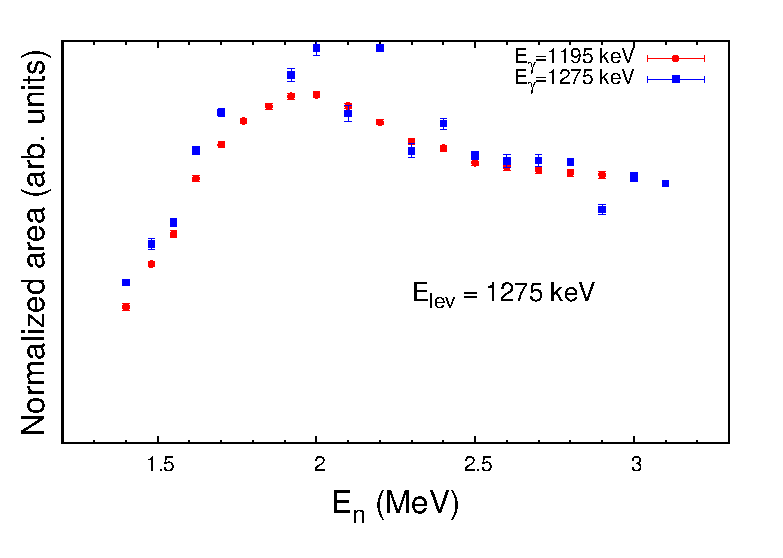
\includegraphics[width=0.75\textwidth]{figures/1195_ExF.eps}\\
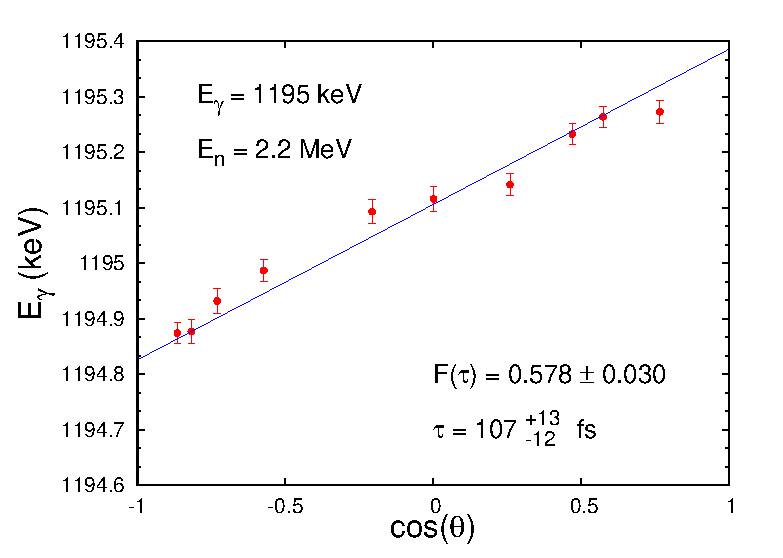
\includegraphics[width=0.49\textwidth]{figures/1195_DSAM.eps}
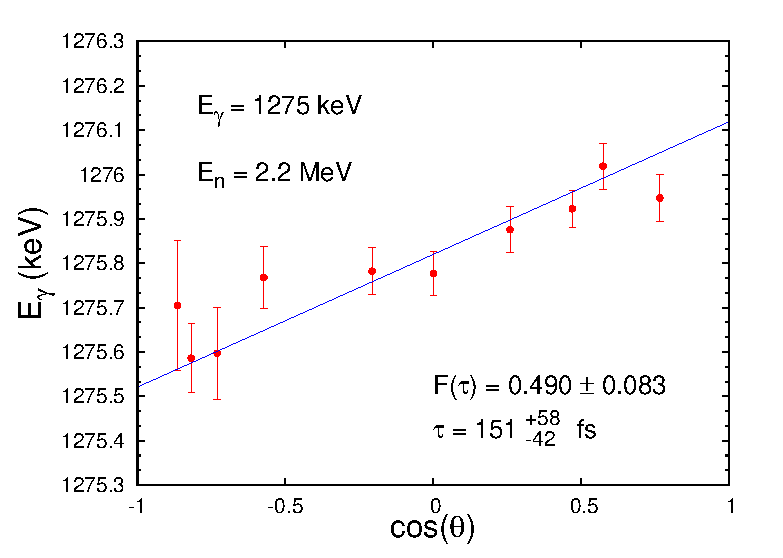
\includegraphics[width=0.49\textwidth]{figures/1275_DSAM.eps}

\caption{E$_\gamma$=1195 \& 1275~keV (de-excitations from the E$_{\rm x}$=1275~keV level) Doppler shifts and excitation functions (color online). The excitation function (in blue) for the 1275~keV $\gamma$ ray is scaled by a factor of 1.53 to normalize to the branching ratio of the level. \label{fig:1275_DSAM_EXF}}
\end{center}
\end{figure}

\begin{figure}[h]
\begin{center}
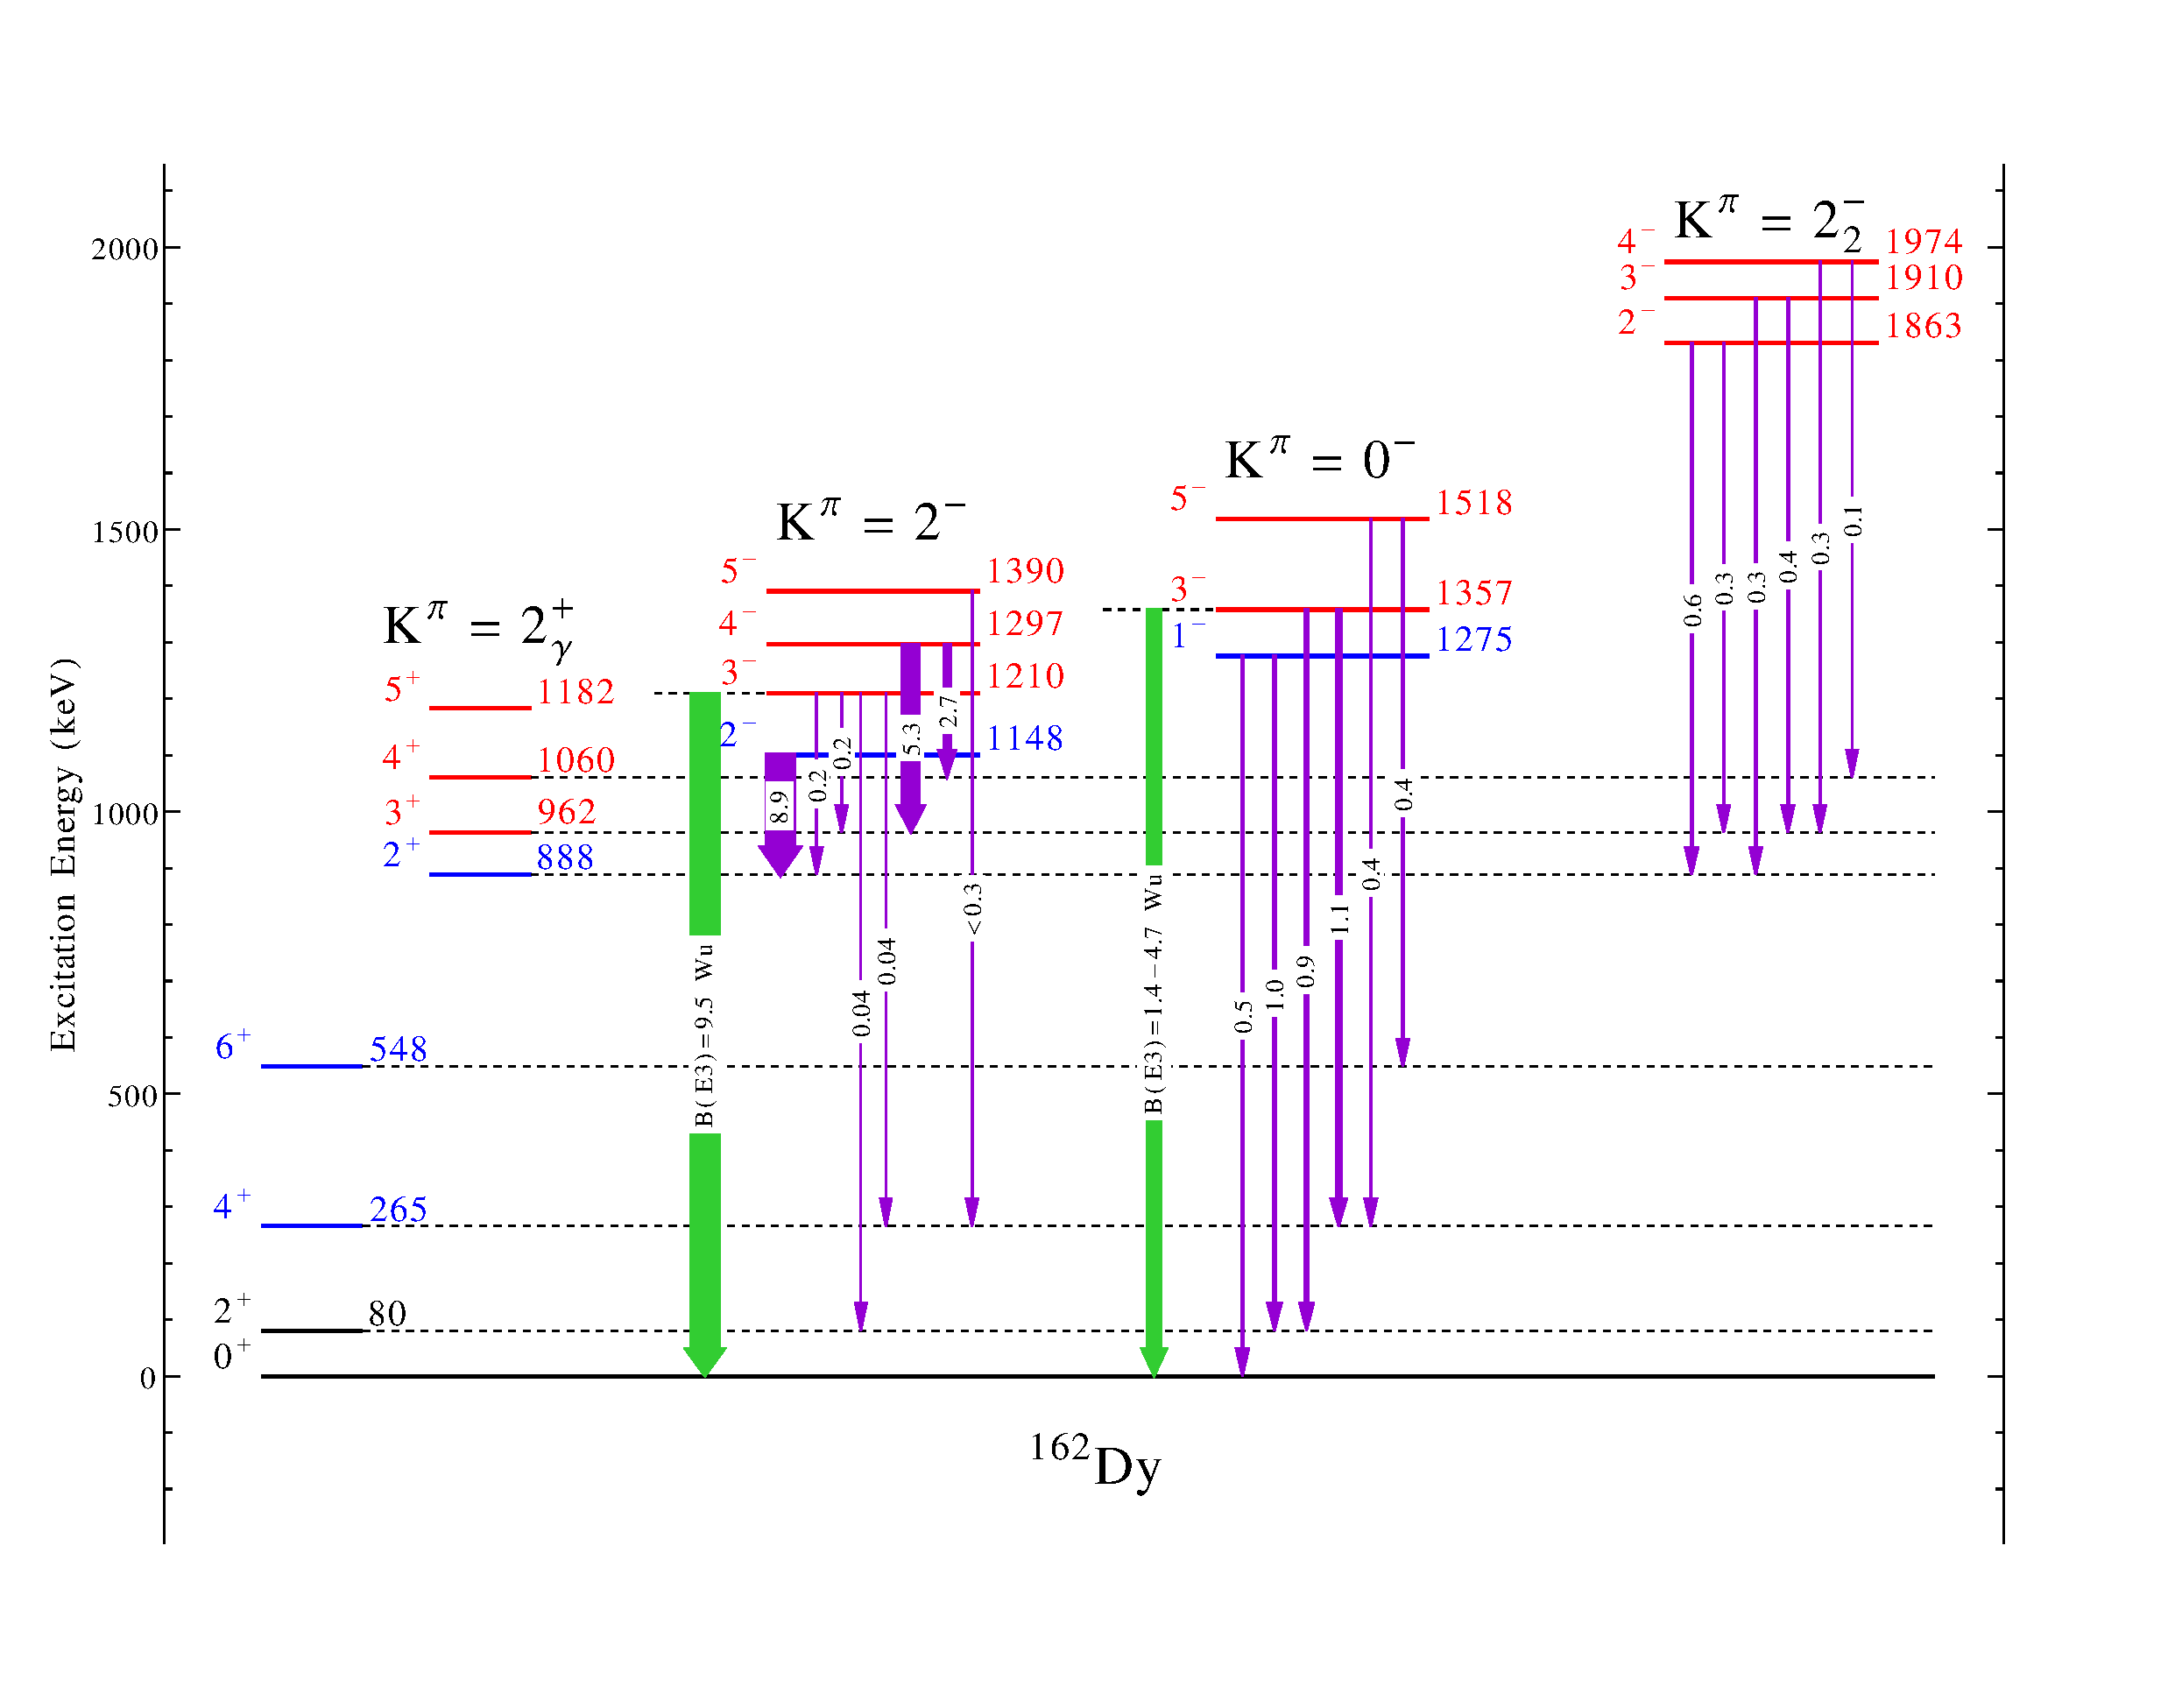
\includegraphics[width=0.98\textwidth]{figures/162Dy_negparity_202.pdf}
\caption{Observed $\gamma$-decays from negative parity, K$^\pi$=2$^-$, 0$^-$, 2$^-_2$ bands in $^{162}$Dy. Transition strengths are drawn proportional in width to their deduced B(E1), with E1 transitions (B(E1) in milli-Weksskopf units) in violet (color online). Literature B(E3) values are drawn in green, expressed in W.u., and are from Refs. \cite{McGowan_BE2_1981,OEHLBERG_BE3} \label{fig:162Dy_negparity_202}}
\end{center}
\end{figure}

\subsubsection{K$^\pi$=2$^-_2$ Band at 1863~keV}

Much like the lower 2$^-$ band, our measurement of mildly inflated B(E1) transition probabilities to the $\gamma$-band is striking, and supports the arguments in numerous works of new, emerging decay patterns \cite{Pascu_octupole_2015,Chakraborty_negparity2012,Spiecker_E1strength} of enhanced E1 transitions to the 2$^+$ band as a differing form of collective dipole excitation built on top of the $\gamma$-vibration. Along the same lines, assertions from IBM considerations with the inclusion of \textit{p} and \textit{f} bosons imply that the structure of the lowest-lying negative parity bands \textit{may not} be of purely collective nature  \cite{Aprahamian200642, Iachello_Arima_IBM}, which supports our experimental findings. Deduced B(E1)s behave well when compared to Alaga considerations (Table \ref{tab:162Dy_negparity_ALAGA}), giving us confidence of correct lifetime measurements. Of particular note, however, is the lower relative B(E1) strength than its lower-energy cousins in the first 2$^-$ band, however, the decays from this band are still above the threshold for what would be considered non-collective. Once again, the interband B(E3) strengths to/from these negative parity bands would be invaluable in the further discussion and feasability of this pattern.

\begin{table}[h!]
% \centering
\begin{center}
 \caption{ABSOLUTE INTENSITIES (NEGATIVE PARITY): $^{162}$DY  \label{tab:162Dy_neg202_intensities}}

\begin{tabular}{l|l|l}
% \begin{tabular}{ccc}
E$_{lev}$ (keV) & E$_\gamma$ (keV) & I$_{\gamma,abs}$ (n,n$^\prime\gamma$)  \\ \hline\hline
 1148.20(20) &  260.16(50) & 658.762(7.577)\\  \hline
 1210.05(18) &  247.27(55) &  38.973(1.420)\\
             &  322.05(51) &  57.699(1.240)\\
             &  944.48(50) & 216.160(3.227)\\
             & 1129.46(50) & 384.769(5.182)\\\hline
 1297.06(27) &  236.09(60) &  43.374(1.380)\\
             &  334.15(50) & 245.585(4.666)\\\hline
 1390.52(35) & 1124.88(88) &  94.848(2.193)\\\hline
 1275.81(24) & 1195.10(50) & 429.944(4.249)\\
             & 1275.82(53) & 280.443(6.356)\\\hline
 1358.00(30) & 1092.27(71) & 134.371(1.271)\\
             & 1277.33(58) & 178.995(6.684)\\\hline
 1518.47(29)&   970.01(55) &  32.453(0.775)\\
            &  1252.74(51) &  78.039(1.893)\\\hline
 1863.85(26)&   900.90(55) &  47.527(1.219)\\
            &   975.65(50) & 141.639(1.587)\\\hline
 1910.50(26)&   947.51(56) &  48.580(0.955)\\
            &  1022.33(53) &  39.474(0.978)\\\hline
 1972.99(66)&   912.09(50) &  82.148(3.125)\\
            &  1010.19(50) & 251.922(15.219)\\\hline
\end{tabular}
\end{center}
Absolute intensities for $\gamma$-decays from the K$^\pi$=2$^-$, 0$^-$, and 2$^-_2$ bands observed in (n,n$^\prime\gamma$) experiments, taken from the E$_n$=3.1~MeV angular distributions.
\end{table}

\begin{table}
\begin{center}
\caption{ALAGA (K$^\pi$=2$^-$,0$^-$,2$^-_2$): $^{162}$DY \label{tab:162Dy_negparity_ALAGA}}
\begin{tabular}{l c c|c}
K$^\pi$ & $\frac{J_{K_i}\rightarrow J^\prime_{K_f}}{J_{K_i}\rightarrow J^{\prime\prime}_{K_f}}$ & Exp & Th \\
\hline
\hline
\underline{K$^\pi_i$=2$^-$:}   & $\frac{3^-\rightarrow3^+_\gamma}{3^-\rightarrow2^+_\gamma}$ & 1.0 & 1.4 \\
                               & $\frac{4^-\rightarrow4^+}{4^-\rightarrow3^+}$ & 0.5 & 0.6 \\ \hline
\underline{K$^\pi_i$=0$^-$:}   & $\frac{1^-\rightarrow2^+}{1^-\rightarrow0^+}$ & 2.0 & 2.0 \\
                               & $\frac{3^-\rightarrow4^+}{3^-\rightarrow2^+}$ & 1.2 & 1.3 \\
                               & $\frac{5^-\rightarrow6^+}{5^-\rightarrow4^+}$ & 1.0 & 1.2 \\  \hline
\underline{K$^\pi_i$=2$^-_2$:} & $\frac{2^-\rightarrow3^+}{2^-\rightarrow2^+}$ & 0.5 & 0.5 \\
                               & $\frac{3^-\rightarrow3^+}{3^-\rightarrow2^+}$ & 1.6 & 1.4 \\
                               & $\frac{4^-\rightarrow4^+}{4^-\rightarrow3^+}$ & 0.3 & 0.6 \\ \hline

\end{tabular}
\end{center}
Comparison of E1 transition probabilities from the K$^\pi$=2$^-$, 0$^-$, \& 2$^-$ bands with the Alaga rules.
\end{table}
%%%%%%%%%%%%%%%%%%%%%%%%%%%%%%%%%%%%%%%%%%%%%%%%%%%%%

